%%%%%%%%%%%%%%%%%%%%%%%%%%%%%%%%%%%%%%%%%%%%%%%%%%%%%%%%%%%%%%%
% rjw 11/25/18 Make subsection of the Validation section 
% 1/9/19 Move back to just after the Introduction.
% rjw 4/7/19 move to appendix per TB
%
\subsection{Simulation}
\label{sec:fdsp-pd-simphys}
%\metainfo{(Length: \dword{tdr}=50 pages, TP=20 pages)}
%\metainfo{\color{blue} Content: Conveners}
% Provided by Alex H. 15mar18
%\metainfo{Content: Himmel}

%Content update by AH nov 2018
%edits by rjw nov 2018

%\forlbnc{LBNC: ``Overall for Section 1.1, I think the technical requirements are clearly explained, but the driving motivations are not.''

%A. The requirements all flow down from the highest level physics goals of the experiment. However, it's somewhat difficult to attach each detector property directly to the physics goals, so these ``physics deliverables'' act as an intermediary. In this chapter we take these as given, and show how we meet them, without needing to get into the detailed physics of different nucleon decay channels or supernova models here. To help make this connection more explicit, we have added references to relevant sections of the physics TDR where these requirements are defined.}

The broad performance specifications for the \dword{pds} are determined by a series of physics deliverables addressing the major physics goals of DUNE: nucleon decay searches, supernova burst neutrinos, and beam neutrinos. Detailed sub-detector specifications, such as light yield of the light collectors, are determined using a full simulation, reconstruction, and analysis chain developed for the \larsoft framework. 

%\fixme{I'm confused: the goals determine the needed sim/reco/analysis work which determines the requirements, which in turn determine the deliverables? Or the goals determine the deliverables, which determine the sim/reco/analysis work, which determines the requirements? Anne}
%The major physics goals of DUNE -- nucleon decay searches, \dword{snb} neutrinos, and beam neutrinos -- determine a series of physics deliverables.  The \dword{pds} requirements flow from the physics needs, determined using a full simulation, reconstruction, and analysis chain developed for the \larsoft framework. 

%The goal is to evaluate the performance in physics deliverables for each of the photon collector designs under consideration. The metrics evaluated will include efficiency for determining the time of the event ($t_0$), timing resolution, and calorimetric energy resolution for three physics samples: \dword{snb} neutrinos, nucleon decay events, %\footnote{The most relevant sample is actually the \emph{background} to nucleon decay events. However, efficiently simulating background that can mimic nucleon decays is challenging since they can be quite rare topologies, so it is easier to simulate the nucleon decay signal which should be representative of the background.}, 
%and beam neutrinos. However, the development of analysis tools to take advantage of this full simulation chain is fairly recent, so this proposal will only include one test case: $t_0$-finding efficiency for \dword{snb} neutrinos versus the effective area of the photon collectors (see Section~\ref{sssec:photoncollectors}).


\subsubsection{Simulation and Reconstruction Steps} 
\label{subsec:fdsp-pd-simphys-sim}

The first step in the simulation specific to the \dword{pds} is the simulation of the production of light and its transport within the volume to the \dwords{pd}. Argon is a strong scintillator, producing \SI{24000}{$\gamma$s/MeV} at our nominal drift field. Even accounting for the efficiency of the \dwords{pd}, it is prohibitive to simulate every optical photon with \dword{geant4} in every event. So, prior to the full event simulation, the detector volume is voxelized and many photons are produced in each voxel. The fraction of photons from each voxel reaching each photosensor is called the visibility, and these visibilities are recorded in a 4-dimensional library.
%rjw 3/19 removed per LBNC (akin to the photon maps used in the \dword{dpmod} simulation described in \voltitledp~Chapter~5).
%\fixme{This reference to DP chapter 5 is hardwired - check this is the correct chapter number.}
This library includes Rayleigh scattering length ($\lambda_R=$ \SI{60}{cm}~\cite{Grace:2015yta}), absorption length ($\lambda_A=$ \SI{20}{m}), and the measured collection efficiency versus position of the double-shift light-guide bars. There is significant uncertainty on the scattering length in the literature, so the value is conservatively chosen at the low end of those reported. With these optical properties, there is a factor of 20 difference in total amount of light collected between events right in front of the photon detectors and those on the far side of the drift volume \SI{3.6}{m} away. 

When a particle is simulated, at each step it produces charge and light. The light produced is distributed onto the various \dwords{pd} using the photon library as a look-up table and the 30\% early (\SI{6}{ns}) plus 70\% late (\SI{1.5}{$\mu$s}) scintillation time constants are applied. Transport time of the light through the \lar is not currently simulated, but is under development. It is not expected to make a significant difference in the studies presented here.

%\forlbnc{LBNC: (previous paragraph) ``...no simulation yet. Can we give a projected impact??"
%A. The more precise timing resolution is not expected to make much impact on the physics shown here. Having it may open up some new possible applications (nucleon decay identification using fine time structure, for example), but those types of applications are still quite speculative so were not included here.}

The second step is the simulation of the sensor and electronics response. For the studies shown here, the SensL \dword{sipm} and \dword{sipm} signal processor (\dword{ssp}) readout electronics used for \dword{pd} development and in \dword{pdsp} is assumed (see Section~\ref{sec:fdsp-pd-pde}). However, a range of \dword{s/n} and dark rates are considered in order to set requirements on the needed performance of the electronics.
%Waveforms are produced on each channel by adding an \dword{sipm} single-\phel response shape for each true photon. In addition, other characteristics of the \dword{sipm} are included such as dark noise, and crosstalk, based on data from device measurements. 
%) From Alex 4/17/18 - We do include afterpulsing as well, at rates based on the sensl sipm's tested in Hawaii. You can just add it to the list of things included in the electronics simulation. 
Crosstalk (where a second cell avalanches when a neighbor is struck by a photon generated internal to the silicon) is introduced by adding a second \phel \num{16.5}\% of the time when an initial \phel is added to the waveform. Additional uncorrelated random noise is added to the waveform with an RMS of %\SI{2.6}{ADC} (or approximately 
\SI{0.1}{\phel{}}. The response of the \dword{ssp} self-triggering algorithm, based on a leading-edge discriminator, is then simulated to determine if and when a \SI{7.8}{$\mu$s} waveform will be read out, or in the case of the simulation, 
stored and passed on for later processing.

%\forlbnc{LBNC: ``where do these numbers come from (for added cross-talk, noise)? Are they ``typical values''  - conservative values?''
%A. These are typical values based on various lab measurements of devices, though they may not all be from the exact same device. However, studies of a wide range of S/N and dark rates showed little impact on physics, though low S/N/ does typically lead to higher data rates.}

The third step is reconstruction, which proceeds in three stages. The first is a ``hit finding'' algorithm that searches for peaks on individual waveforms channel-by-channel, identifying the time (based on the time of the first peak) and the total amount of light collected (based on the integral until the hit goes back below threshold). The second step is a ``flash finding'' algorithm that searches for coincident hits across multiple channels. All the coincident light is collected into a single object that has an associated time (the earliest hit), an amount of light (summed from all the hits), and a position on the plane of the \dword{apa} ($y$-$z$) that is a weighted average of the positions of the photon collectors with hits in the flash. %\footnote{Currently, the flash reconstruction does not consider the positions of the hits, only their times. This will need to be updated in the future when we simulate the full-sized \dword{spmod} but for now we are working in a small test geometry that acts as a crude simulation of this kind of constraint.}. 
The final step is to ``match'' the flash to the original event by taking the largest flash within the allowed drift time that is within \SI{240}{cm} in the $y$-$z$ plane. Since the TPC reconstruction is still in active development, especially for low-energy events, we match to the true event %\dword{mc} 
vertex of the event in the analyses presented here. This is a reasonable approximation since the position resolution of the TPC will be significantly better than that of the \dword{pds}. 

These tools (or subsets of them) are then used to evaluate how the performance of the \dword{pds} affects the following set of physics deliverables.

\subsubsection{Nucleon Decay}
\label{subsec:fdsp-pd-simphys-ndk}

Nucleon decays are rare events, so excluding backgrounds is of the utmost importance. Since some backgrounds can be generated by cosmic rays passing outside the active detector area, setting a fiducial volume to exclude such events is critically important.

\textit{Fiducialization with \tzero}\nopagebreak

%The following LBNC comment was specific to nucleon decay but is more generally in the way we use the term "physics deliverable"
%\forlbnc{LBNC: ``it's not clear why this is the ``physics deliverable'' - the physics deliverable is presumably - ``we want to have sensitivity to x nucleon decay''. That then drives that we have to be able to see 99\% of such decays in the detector, which in turn drives the light yield requirements.''
%A. This is a concrete instantiation of the requirement laid out in the Nucleon Decay chapter of the Physics TDR. We have added an explicit reference to this section.}

The physics deliverable: the \dwords{pd} must be able to determine \tzero with approximately \SI{1}{\micro s} resolution (SP-FD-4: time resolution) for events with visible energy greater than \SI{200}{MeV} throughout the active volume, and do so with $>99\%$ efficiency (SP-FD-3: light yield), as described in Section~\ref{subsec:nonaccel-ndk-requirements}. 
%Note this subsec reference is in the physics volume so will show as ??? when one chapter is compiled alone.
This energy regime is relevant for nucleon decay and atmospheric neutrinos. The time measurement is needed for event localization for optimal energy resolution and rejection of entering backgrounds. 
This resolution is required for comparable spatial resolution to the TPC along the drift direction.

%\forlbnc{LBNC: ``is efficiency averaged over the entire detector? Or just in the dimmest regions? The CPA is an important reference point because it is the farthest point from the PDS?''
%A. This is light yield at the CPA, the dimmest region of the detector. We have added additional explanation to the caption to make this point clear.}

\begin{dunetable}[PD system efficiency for nucleon decay events]
{ccc}
{tab:pds-ndk}
{Efficiency for tagging nucleon decay events with the \dword{pds} at the \dword{cpa}, the dimmest region of the detector, which is \SI{3.6}{m} from the \dwords{pd}, shown for range of light yields (LY) at that position. Also shown is the total PD module collection efficiency required for that light yield with the simulated scattering length, \SI{60}{cm}.)}
\dword{cpa} Light yield (PE/MeV) & Collection Efficiency  (\%) & Efficiency at the \dword{cpa} (\%) \\
%(PE/MeV) & (\%) & (\%) \\ 
\toprowrule
0.09 & 0.24   & $93.8 \pm 0.4$ \\ \colhline
0.28 & 0.75  & $97.7 \pm 0.4$ \\ \colhline
0.33 & 0.88  & $98.4 \pm 0.2$ \\ \colhline
0.50 & 1.3  & $98.9 \pm 0.2$ \\ 
\end{dunetable}


The physics here feeds down to a requirement on the minimum light yield (SP-FD-3: light yield), determined by measuring how often the correct flash was not assigned to nucleon decay 
events\footnote{The most relevant sample is actually the \textit{background} to nucleon decay events. However, efficiently simulating background that can mimic nucleon decays is challenging since they can be quite rare topologies. It is therefore easier to simulate the nucleon decay signal that should be representative of the background.} 
in the dimmest region of the detector, near the \dword{cpa}. A minimum light yield of \SI{0.5}{PE/MeV} is required to meet the requirement of 99\% efficiency, as shown in Table~\ref{tab:pds-ndk}. 

A light collector with 1.3\% collection efficiency (defined as the probability that a photon reaching the surface of the light collector will be recorded as a \phel) achieves this light yield with the simulated \SI{60}{cm} scattering length. This efficiency is equivalent to having \SI{23}{cm^2} of active area per module with 100\% efficiency. At this scattering length there is a factor of 20 difference in light yield between the brightest and dimmest regions of the detector, so techniques to improve light yield uniformity (discussed in Appendix~\ref{sec:fdsp-pd-enh}) would reduce the inefficiency still further and ease understanding the detector systematic uncertainties.


\subsubsection{Supernova Neutrinos}
\label{subsec:fdsp-pd-simphys-snb}

Supernova bursts are also rare events, though here the event is made up of many interactions (spread over several seconds) instead of a single interaction. For distant supernovae (at the far side of the Milky Way or in the Large Magellanic Cloud), the top priority is to ensure that the detector can identify a burst when it happens and trigger the detector readout. For nearby supernovae, triggering will not be a challenge, and instead the goal is to record as much information as possible about the burst.

\textit{Burst Triggering}\nopagebreak
%\forlbnc{LBNC: ``this is closer to a physics deliverable in my mind - we have to be able to see SNBs in our galaxy and the LMC. It's not clear, however, why the PDS trigger needs similar performance to the TPC trigger.''
%A. Missing a supernova would be a serious problem for DUNE. So, we require redundant triggering abilities. By having two highly capable triggering systems in each single phase module, we dramatically reduce the chance of missing a supernova, even if one system or the other is unable to trigger because of some adverse detector conditions (for example: poor purity or on-going calibration). In order to make this point clear, we are changing to text to give a specific target for efficiency, before discussing similarity to the TPC.}

The physics deliverable: the \dword{pds} must be able to trigger on \dwords{snb} which produce 50 neutrino interactions in a \SI{10}{kt} volume\footnote{About the amount expected for a burst at the far side of our galaxy.} with almost 100\% efficiency with a false positive rate of less than one per month. This deliverable is most important for distant supernovae where the most important requirement is that we trigger and record the data. If both the \dword{pds} and TPC triggers have good efficiency, they can provide redundancy against one another or be combined to increase efficiency or lower the background rate. The once-per-month false positive rate is determined by limits in data handling.

%\forlbnc{LBNC: (last sentence previous para) ``in my reading of the DAQ, I got no sense of a limit? What do PDS know that we don't??''
%A. This was a benchmark value given to us when developing trigger plans, which I believe is more related to total data volume limitations than DAQ, so if we can do some relatively fast analysis on the burst we can likely tolerate a higher false positive rate, but without having any other concrete guidance we decided to stick with this conservative benchmark.}

The \dword{pds} trigger performance was studied for a plausible but challenging signal: a supernova burst in the Large Magellanic Cloud, which we conservatively assumed would produce only 10 signal events in the far detector. The trigger efficiency was studied with variations in light yield, dark rate, and signal-to-noise ratio, keeping the requirement from the DAQ that the fake rate be held to less than one per month. The burst trigger efficiency for 10 supernova neutrino events in one \SI{10}{kt} module (a  pessimistic prediction for a supernova in the LMC), was found to be approximately $80\%$, and it is relatively insensitive to all these parameters for average light yield $>$\SI{7}{PE/MeV} (equivalent to 0.9\% collection efficiency with the simulated optical properties), dark rate $<$\SI{1}{kHz}, and signal-to-noise $>3$. The uncorrelated noise from dark rate and low signal-to-noise was easily excluded from trigger primitives by the clustering scheme, and the increased light yield makes both backgrounds and signal brighter together so performance stays basically constant. Thus this physics deliverable, while important, does not constrain any detector requirements.


\textit{TPC Energy Measurement and Time Resolution with \tzero}\nopagebreak

%\forlbnc{LBNC: ``same comment on ``physics deliverable'' - this is a technical requirement driven by a higher physics deliverable that isn't listed here. I'll stop making these comments from here on out.''
%A. We believe discussing the details of supernova physics is out-of-scope for the PDS chapter, so we are adding a reference to the SNB physics chapter where the benefits of increased energy resolution are discussed.}

The physics deliverable: the \dwords{pd} must be able to provide \tzero determination with \SI{1}{\micro s} resolution (SP-FD-4: time resolution) for at least 60\% of the neutrinos in a typical \dword{snb} energy spectrum. The \tzero measurements are used in concert with the TPC-reconstructed event in two ways: to correct for the attenuation of the charge signal as a function of how far the charge drifts through the TPC and to provide more precise absolute event times for resolving short time features in the \dword{snb} neutrino event rate. This deliverable is important primarily for nearby supernovae where the number of events is large enough that time and energy resolution will be the limiting factors in extracting physics, as described in Section~\ref{sec:physics-snblowe-detector-requirements}. 

\begin{dunefigure}[Supernova neutrino energy resolution from the TPC]
{fig:pds-snb-driftcor}
{The energy resolution for supernova neutrino events when reconstructed by the TPC with the drift distance corrected using three assumptions on the performance of the \dword{pds}. The options considered range from drift correction for no events (black), to 60\% of events (blue), to 100\% of events (red).
}
  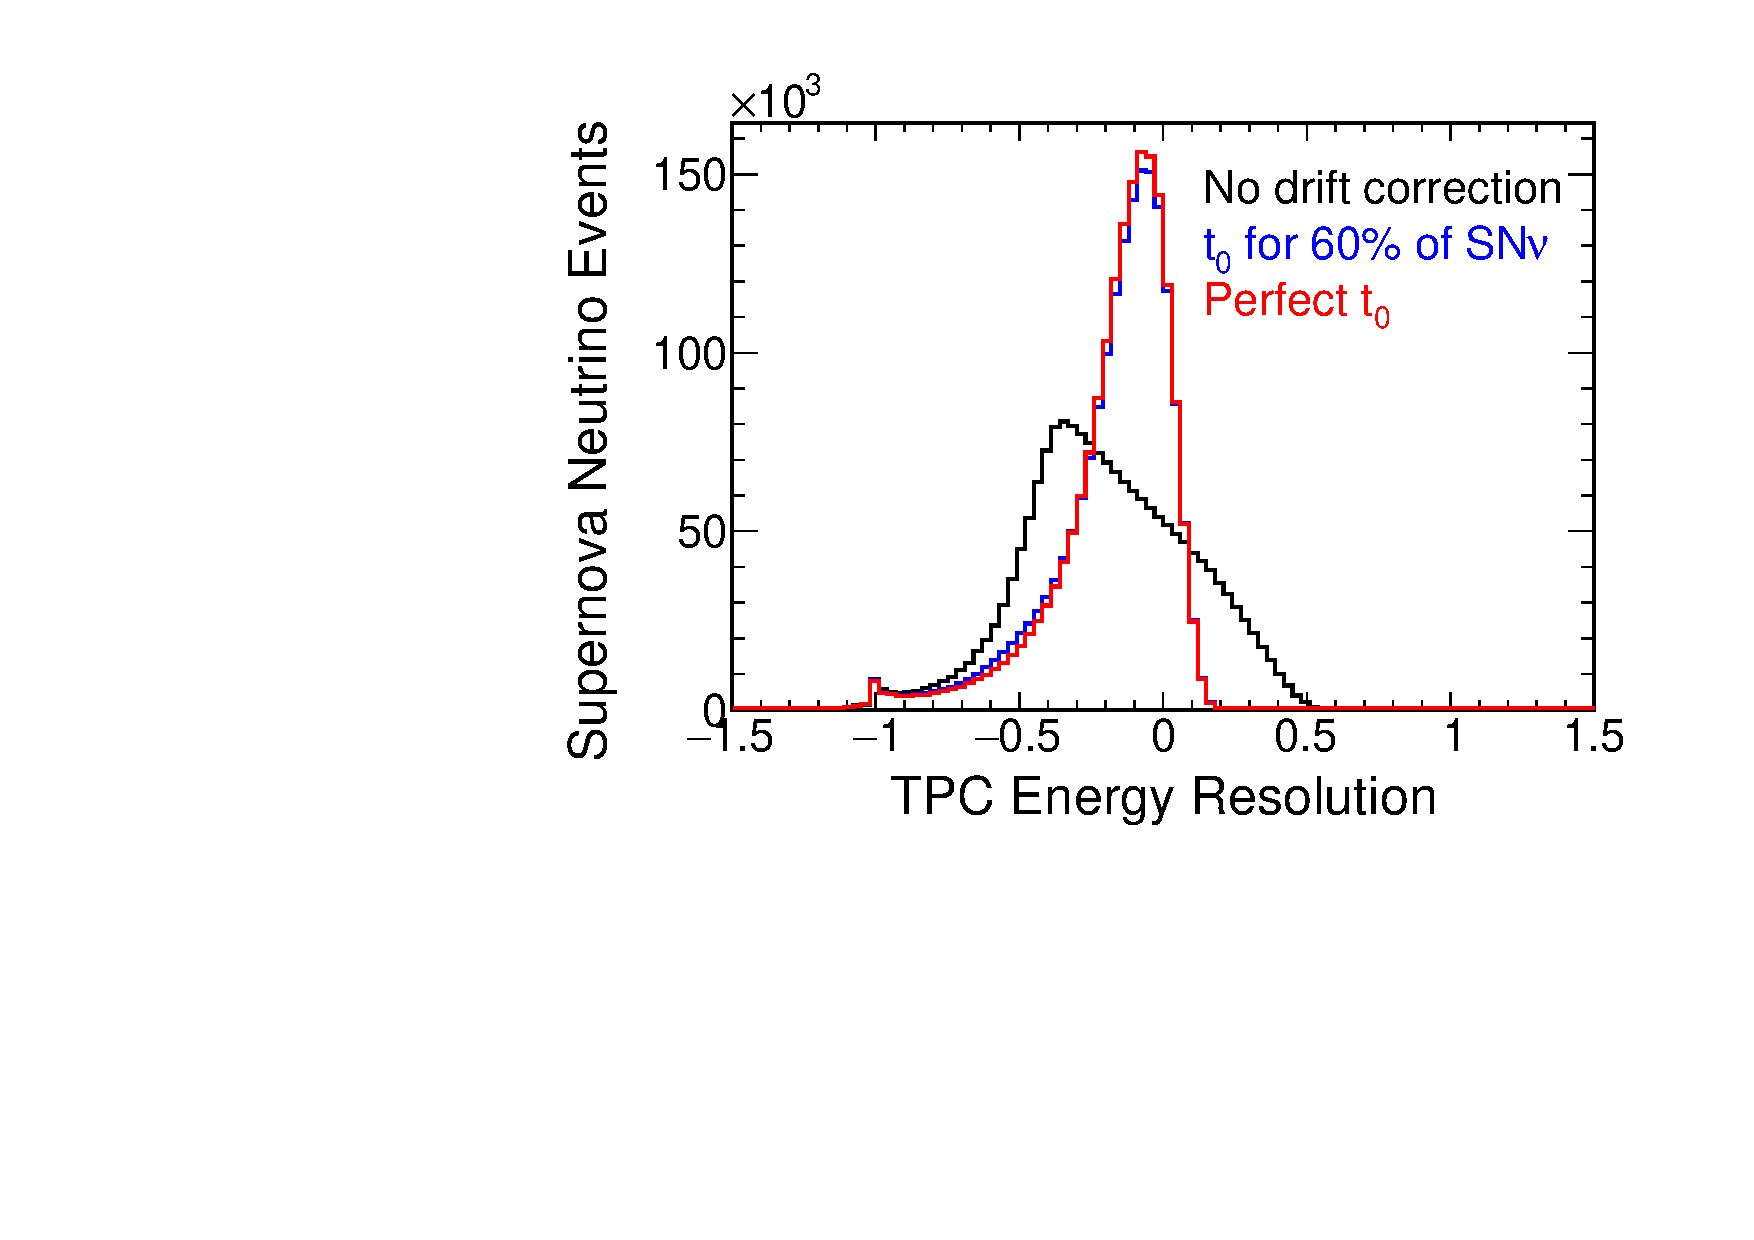
\includegraphics[width=0.5\textwidth]{graphics/pds-snb-drift-corr}
 \end{dunefigure}

The 60\% \tzero tagging requirement comes from two studies of a typical \dword{snb} neutrino spectrum under varying \dword{pd} performance assumptions: the resolution of the energy reconstructed with the TPC and drift-corrected using the time from the \dwords{pd}, and the observability of the in-fall `notch' in the \dword{snb} event time distribution. Both studies show significant improvement when going from no \dwords{pd} to a system that has a collection efficiency of at least 0.25\% (equivalent to \SI{0.5}{PE/MeV} for 60\% of the detector volume), but only marginal improvements past that point, as can be seen in Figure~\ref{fig:pds-snb-driftcor}. The light yield required here is sufficiently low that this deliverable does not set any additional detector requirements.


\textit{Calorimetric Energy}\nopagebreak

Physics deliverable: the \dword{pds} should be able to provide a calorimetric energy measurement for low-energy events, like \dwords{snb}, complementary to the TPC energy measurement. 
Improving the energy resolution will enable us to extract the maximum physics from a \dword{snb} (see Section~\ref{sec:physics-snblowe-detector-requirements}), and with the goal to achieve energy resolution comparable to the TPC, we can take full advantage of the anti-correlation between the emission of light and charge signals imposed by the conservation of energy. In addition, this requirement allows the photon detection system to provide redundancy if a supernova occurs during adverse detector conditions. If the argon purification system is offline, the photon signal is significantly less sensitive to electronegative impurities, and if the drift field is low, the reduced charge signal can be partially recovered by increased light.
%\forlbnc{LBNC: ``Calorimetric energy, simulations in Fig 1.2. Do these results come from just one simulation. Is there more than one simulation? Is there agreement between simulations?'' 
%A. The physics studies are all based on one simulation implemented in LArSoft. The lines on this plot were made with different assumptions about the efficiency of the detectors, but come from the same underlying simulation.}

%\forlbnc{LBNC: ``Figure 1.2 - why didn't you try 23 cm$^2$ as a case, which was the area driven above? i feel that the physics case here overall is still not clear enough to me.  The first paragraph here states that the PDS should provide complementary energy info to the TPC to “extract maximum physics” but again, there's no actual physics plot that states what that 'maximum' physics is for a resolution of 0.3 vs. 0.4.  That study might be in the Physics TDR but it needs to exist and be referenced.''
%A. The MC runs at different light yields are fairly costly, and the range of values we were interested in testing has changed over time (the nucleon decay studies were done before the supernova studies). However, it is straightforward to interpolate between light yields. As with the other comments along these lines, we are adding cross-references to the physics chapters rather than trying to address the details of supernova physics here in the photon detector chapter.}

\begin{dunefigure}[SNB neutrino energy resolution from the PD system]
{fig:pds-snb-calo}
{The energy resolution (determined from the distribution widths of the fraction of difference between reconstructed and true to true neutrino energy for simulated events) for supernova neutrino events when reconstructed directly through \dword{pds} calorimetry for a range of light yields, represented by different colors. The red line labeled \textit{Physics} 
shows the energy smearing inherent to the neutrino interactions and thus serves as a theoretical minimum resolution. The black line shows the energy resolution achieved by the \dword{tpc}, defined in a similar way. The performance improves significantly up until approximately \SI{20}{PE/MeV} where the \dword{pds} and \dword{tpc} give comparable resolution below approximately \SI{7}{MeV}.
%The behavior vs. true and reco energy looks different because some higher energy neutrinos lose otherwise visible energy into neutrons, causing the poorly resolved higher true energy events to all feed down to lower reconstructed energies. 
}
  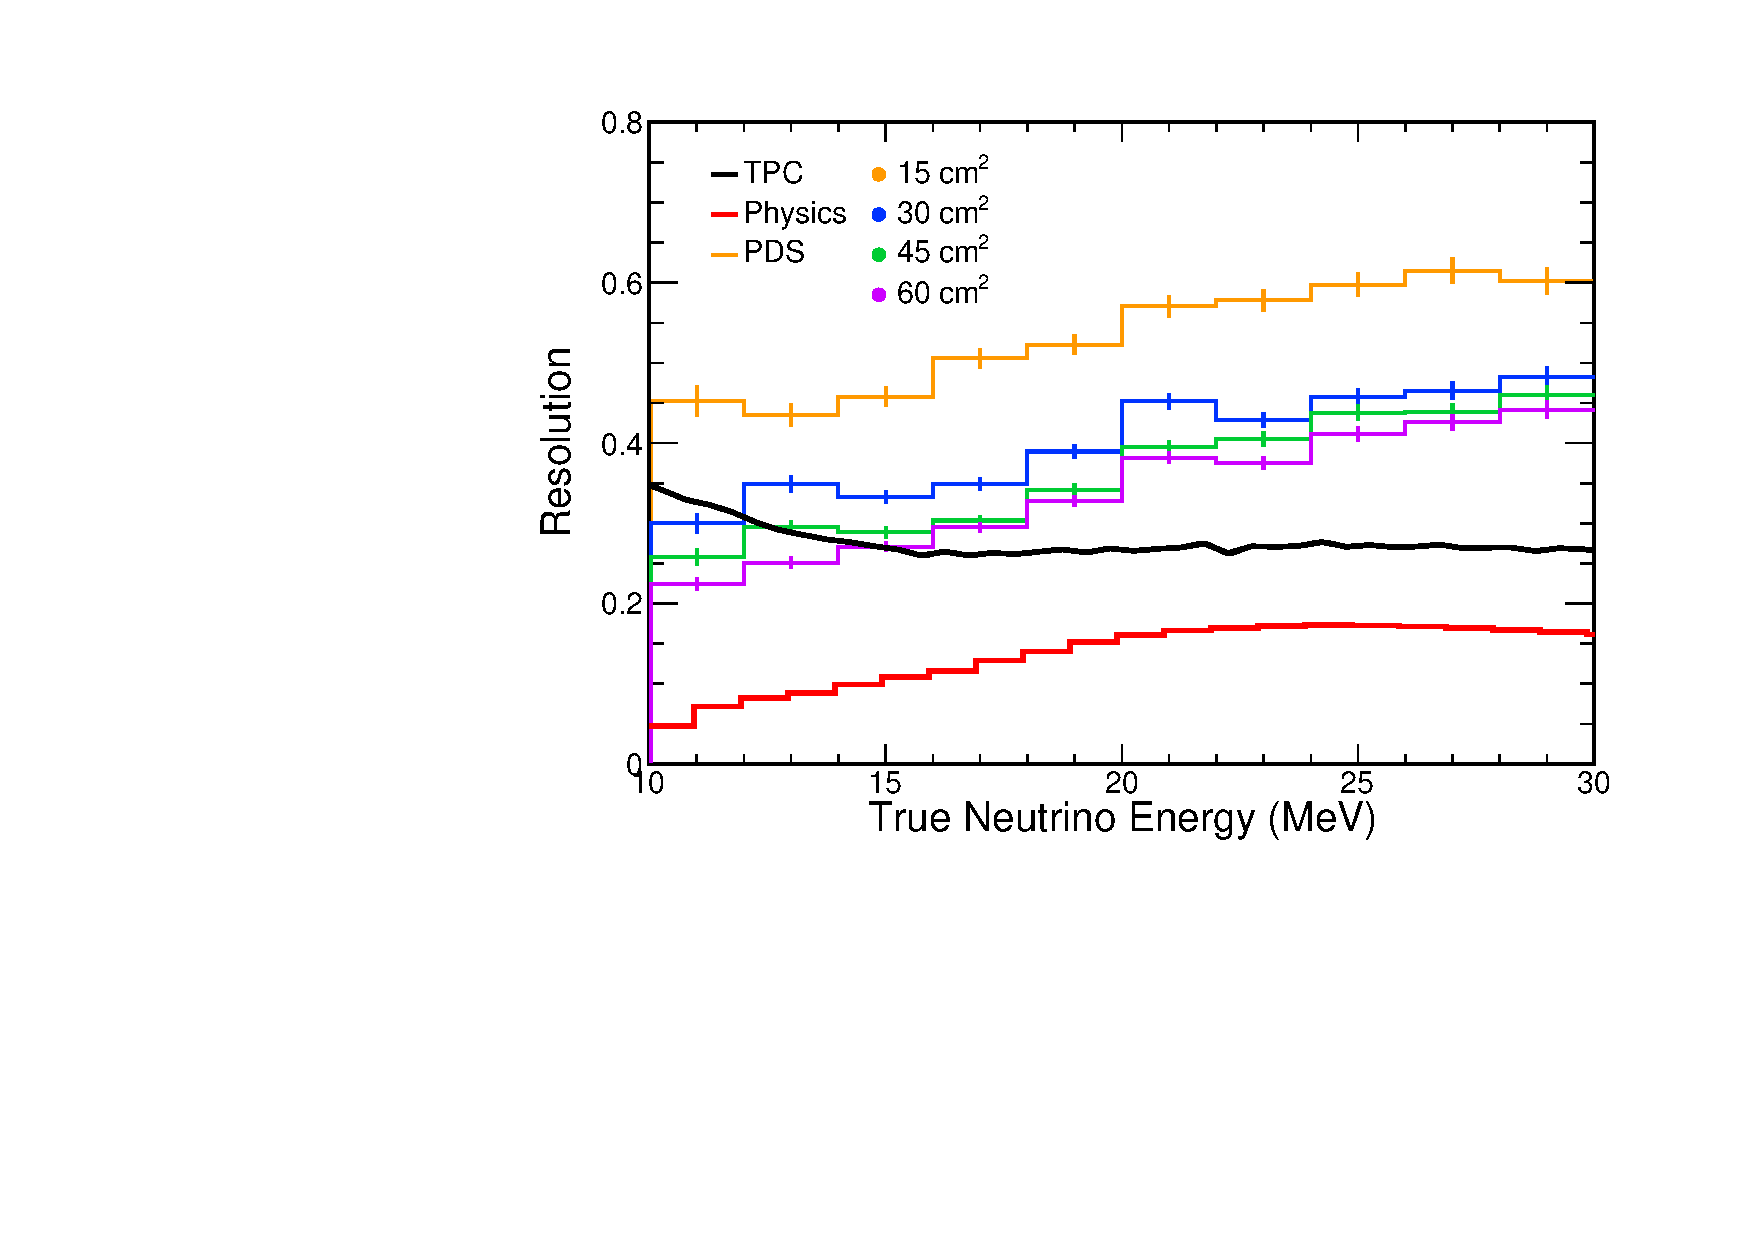
\includegraphics[width=0.6\columnwidth]{graphics/pds-snb-res-vs-true.pdf}
  %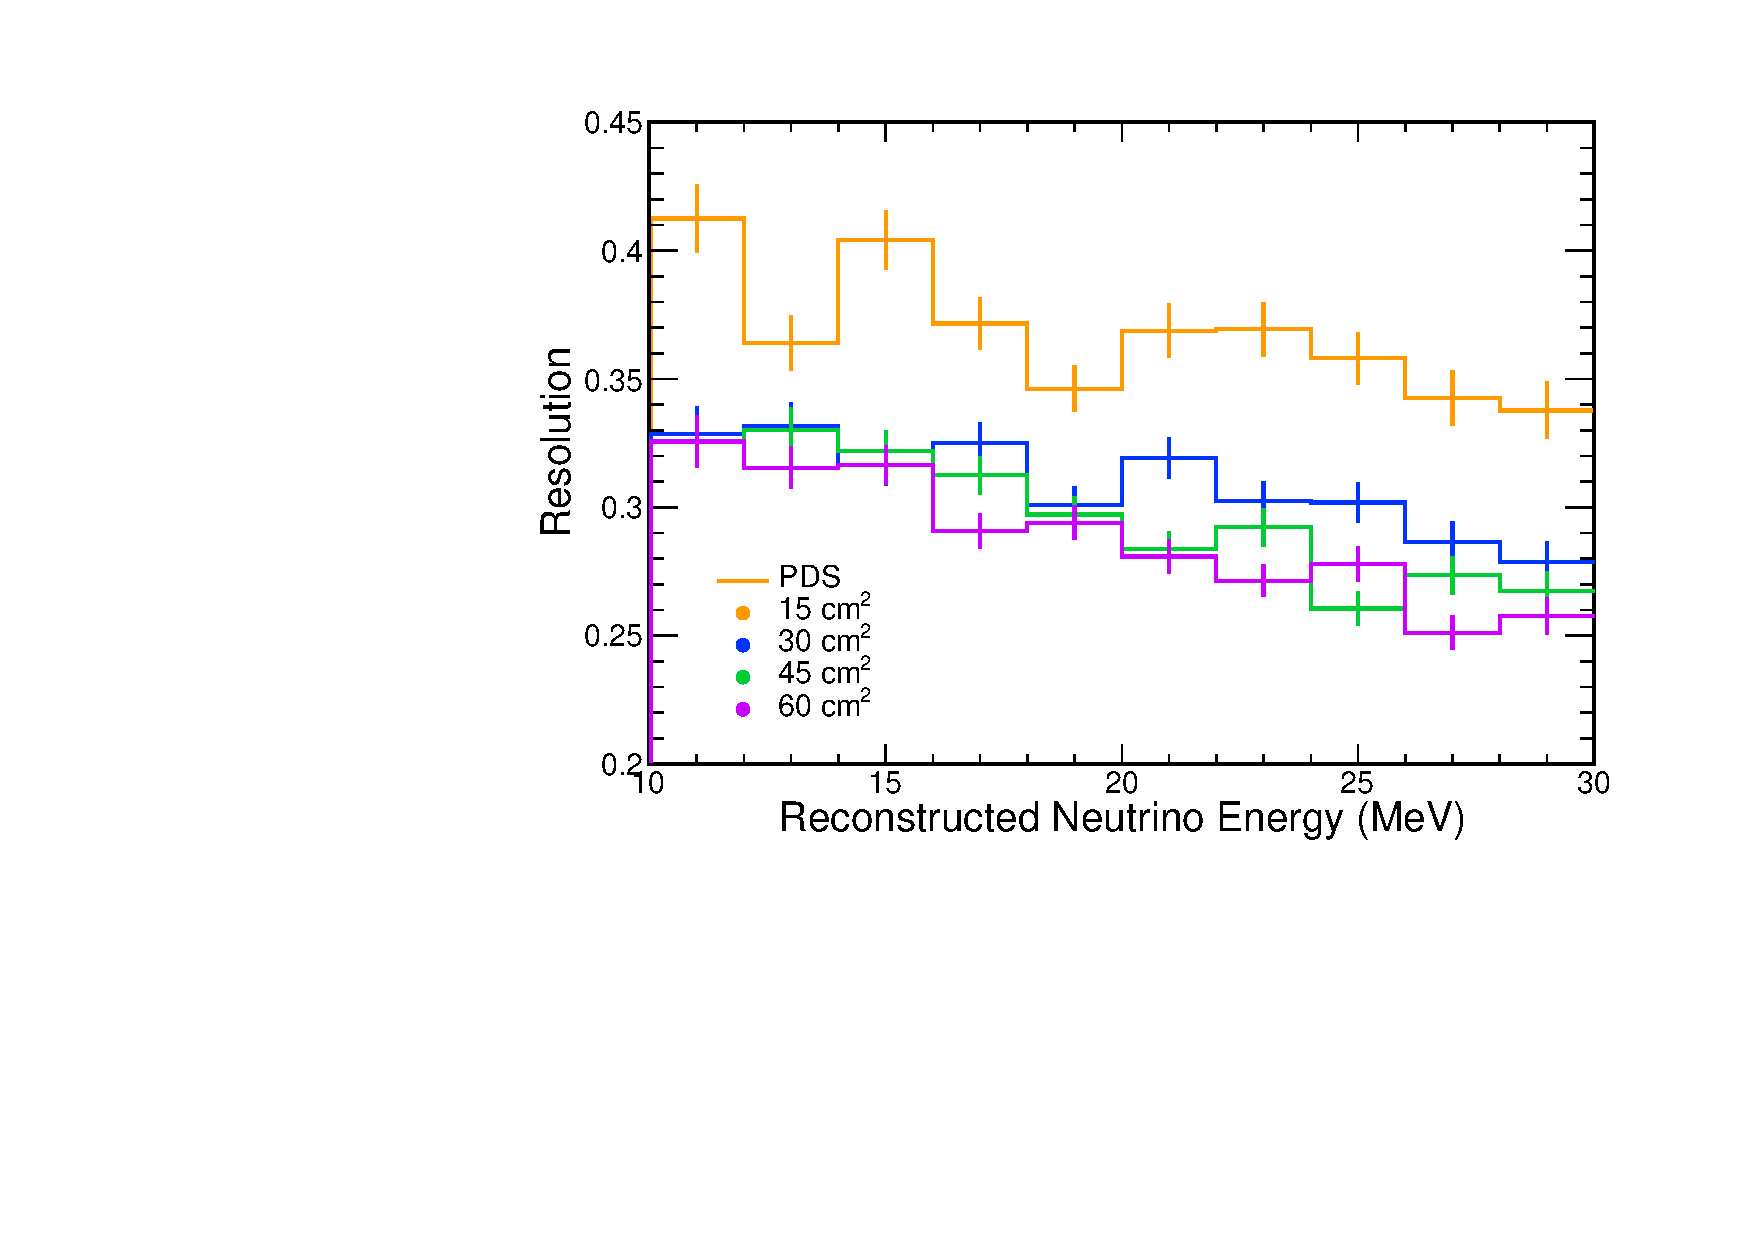
\includegraphics[width=0.48\columnwidth]{graphics/pds-snb-res-vs-reco.pdf}
 \end{dunefigure}

The calorimetric energy performance was studied for supernova burst neutrino events simulated in the far detector for a range of different detector performance assumptions. The energy reconstruction was simple, correcting the total observed amount of photons for the average number of photons expected per MeV as a function of position along the drift direction. Events were required to be well away from the side walls to avoid any possible edge effects. The energy resolution vs. true energy is shown in Figure~\ref{fig:pds-snb-calo}. There is a significant benefit to achieving a photon detector with an average light yield of \SI{20}{PE/MeV}, where the \dword{pds} and \dword{tpc} have comparable resolution for the lowest energy ($<$\SI{7}{MeV}) supernova neutrinos. Past this light yield, the improvement appears to plateau in this analysis. This physics deliverable thus sets a requirement, FD-SP-3: light yield, of \SI{20}{PE/MeV} averaged over the active volume.

While options that can improve the uniformity of the detector are not essential to achieve required resolution, they are likely to improve the calorimetric energy reconstruction above and beyond total light yield. A detector that is more uniform will be easier to calibrate, and the impact of uncertainties on the optical parameters of the liquid argon will be reduced. This effect is potentially important for supernova neutrinos, and certainly more important for the beam neutrino events described in the next section. In addition, for Xe-doping specifically, speeding up the late light will allow for flashes that are narrower in time, reducing the amount of radiological contamination mixed in with the signal, which is of particular importance with these relatively small signals.



\subsubsection{Beam Neutrinos}
\label{subsec:fdsp-pd-simphys-beam}

The \dword{pds} is not required for fiducializing beam neutrino events since the pulsed beam will provide sufficient precision to place the interactions in space. However, the \dwords{pd} can potentially contribute to the energy measurement and the better timing resolution can help identify Michel electrons from muon and pion decay.


\textit{\it Calorimetric Energy}\nopagebreak

Physics deliverable: the \dword{pds} should be able to provide a calorimetric energy measurement for high-energy events, like neutrinos from the \dword{lbnf} beam, complementary to the TPC energy measurement.
Neutrino energy is an observable critical to the success of the oscillation physics program (see Section~\ref{sec:nu-osc-09}), and a second independent measurement can provide a cross-check that reduces systematic uncertainties or directly improves resolution for some types of events. 

In order to provide a meaningful cross-check, the resolution and uncertainty of the \dword{pds} measurement must be comparable to the calorimetric resolution of the TPC. The limit on this measurement will likely come from how well the efficiency of the detector and the optical properties of the argon can be determined (both must be known to approximately 5\% to have a comparable measurement of electron shower energy), which define a program of measurements between now and the operation of the detector rather than requirements on the system itself. The requirement that does flow down from this is that the dynamic range of the system be sufficient to allow for accurate measurement of the amount of light reaching the \dword{pds}. 

%\forlbnc{LBNC: ``again, where does this 20\% number come from? Why is 20\% ok but not 40\%?  although i suppose in the end it doesn't matter since it doesn't saturate anyway according to your sims.''
%A. Unfortunately, we only have a fairly rough estimate of how much saturation we will be able to correct for since this analysis is still on-going. If we find that the saturation is an issue with the X-ARAPUCA design and 12-bit ADCs, it is possible to upgrade the electronics to 14-bit where saturation will, indeed, be negligibly rare for beam events.}

Some amount of saturation is tolerable since it can be corrected for using the pulse shape or the neighboring unsaturated channels. However, if the saturation is too large, and too many channels are saturated, the corrections become difficult, so we require that no more than $20\%$ of beam neutrino events have saturating channels (SP-PDS-16: dynamic range), consistent with but looser than the \dword{tpc} requirement of $10\%$.

We studied the likelihood of channels saturating by simulating beam neutrino events in the far detector. The likelihood of saturation depends on the digitization frequency, the dynamic range, and the collection efficiency of the detector design. Assuming the baseline electronics, a 12-bit and \SI{80}{MHz} digitizer, we find the likelihood of saturation vs. average light yield shown in Table~\ref{tab:pds-dynamicrange}. 

\begin{dunetable}[Fraction of beam events with channels that saturate]
{ccc}
{tab:pds-dynamicrange}
{The fraction of beam events which have saturating \dword{pds} channels for different light yields, and the corresponding \dword{pds} collection efficiencies.}
Avg. Light Yield (PE/MeV) & Collection Efficiency (\%) & Saturation Fraction (\%) \\ \toprowrule
6 & 0.88  & 6 \\ \colhline
13 & 1.8   & 13 \\ \colhline
21 & 2.6   & 20 \\ \colhline
28 & 3.5   & 24 \\ 
\end{dunetable}


\textit{\it Michel Electron Tagging}\nopagebreak

Physics deliverable: the \dword{pds} should be able to identify events with Michel electrons from muon and pion decays.
The identification of Michel electrons can improve background rejection for both beam neutrinos and nucleon decay searches. 
Some Michel electrons are difficult to identify with the TPC since they appear simultaneous within the time resolution of the TPC and colinear with their parent. However, because the \dword{pds} can observe the fine time structure of events in the detector, it can identify Michel electrons that appear separated in time from the main event. While DUNE-specific studies of Michel electron tagging have not been performed, the LArIAT experiment has demonstrated that Michel electrons can be identified and studied using photon signals. 

%\fixme{Add LArIAT reference once it exists}

